\input{preamble_amsart}

\usepackage{lipsum}
\usepackage{textcomp}
\usepackage{esvect}
%\usepackage{chngcntr}
%	\counterwithout{equation}{section}		% Continuous equation numbering throughout document

\setcounter{MaxMatrixCols}{20}				% Change maximum number of matrix columns

\renewcommand{\descriptionlabel}[1]{		% Change description label from "#1:" to "#1."
	\hspace\labelsep\upshape\bfseries #1.
}

%===========================================================================================%
\def\mwmwh{\delta}
\def\eff{\eta}

%===========================================================================================%
% BIBLIOGRAPHY
\usepackage[authoryear, round]{natbib}
	\renewcommand{\bibfont}{\normalfont\small}	%Bibliography font size = small
	
%===========================================================================================%
\hyphenation{allow assumes control demand energy operator}

%===========================================================================================%
\title[Dispatchability of Wind Power with Battery Energy Storage in SA Using MPC]{Dispatchability of Wind Power with\\Battery Energy Storage in South Australia\\Using Model Predictive Control}

%\author{Silvio Tarca$^1$}
%\address{$^1$School of Mathematical Sciences, University of Adelaide}
%\author{Nesimi Ertugrul$^2$}
%\address{$^2$School of Electrical and Electronic Engineering, University of Adelaide}
%\email{silvio.tarca@adelaide.edu.au, nesimi.erutgrul@adelaide.edu.au}
\email{silvio.tarca@adelaide.edu.au}

\date{\today}

%===========================================================================================%
\begin{document}

\maketitle

%===========================================================================================%
% ABSTRACT																					 %
%===========================================================================================%
\begin{abstract}
The Government of South Australia (SA) has pledged to increase the state's electricity generation from renewable energy sources from 41\% in fiscal year 2015 --- 34\% wind and 7\% solar photovoltaic --- to 50\% by 2025.  At these levels of intermittent renewable energy penetration the challenge is to economically supply baseload power of acceptable quality.  We measure the improvement in the dispatchability of intermittent renewable energy from an SA wind farm with battery energy storage using state-space model predictive control (MPC) and real-world data published by the Australian Energy Market Operator.  The process dynamics of wind power dispatch with battery energy storage are formulated as an incremental state-space model, which allows the MPC controller to penalise control effort.  Moreover, the state-space model properly accounts for the charge/discharge efficiency of the battery.  
\end{abstract}

%===========================================================================================%
% INTRODUCTION																				 %
%===========================================================================================%
\section{Introduction}\label{sect:introduction}
The Paris Climate Agreement, negotiated in December 2015, to limit global temperature rise to 2 \textcelsius{} above pre-industrial levels promotes an aggressive transition from fossil fuels to renewable energy sources.  The International Energy Agency \citeyearpar[IEA,][]{IEA15} reports that electricity was 18.0\% of global energy consumption in calendar year 2013, with 67.4\% of global electricity generation coming from the combustion of fossil fuels.  With the transport sector accounting for 27.6\% of global energy consumption in 2013, electricity's share is set to rise markedly as plug-in electric vehicles displace internal combustion vehicles.

The Australian Energy Market Operator \citeyearpar[AEMO,][]{SAER15}, the independent system operator of the National Electricity Market (NEM),\footnote{
The NEM is one of the world's longest interconnected power systems stretching 5,000~km from Port Douglas in Queensland to Port Lincoln in South Australia with 40,000~km of transmission lines \citep{AEMO14a}.  With installed capacity exceeding 51,000~MW the NEM supplied approximately 180,000~GWh of electricity to industrial, commercial and residential customers in fiscal year 2015 \citep{ESOO15, NEFR15}.
} reports that in fiscal year 2015,\footnote{
The Australian fiscal year ends June 30 and is identified by the calendar year in which it ends.  Hence, fiscal year 2015 refers to the period from 1 July 2014 to 30 June 2015.
} 41\% of 12,352 GWh of electricity generated in the state of South Australia (SA) came from intermittent renewable sources --- 34\% wind and 7\% solar photovoltaic (PV).  Through fiscal year 2015 the SA government had already invested AUD 6.6 billion in renewable energy, and plans to increase its investment to AUD 10 billion to achieve its target of 50\% renewable energy generation by 2025 \citep{SAGOV15}.  With the closure of SA's last two ageing coal-fired power plants in May 2016, it now seems likely that SA will reach its renewable energy generation target well in advance of 2025.  Compared to other leading international jurisdictions for renewable energy, SA ranks second (33\% in calendar year 2014) behind Denmark (39\%) on the share of electricity generation from wind, and second (340 Watts) behind Germany (474~Watts) on installed capacity of solar PV per capita \citep{SAGOV15}.  SA is a real-world laboratory for the study of intermittent renewable energy technology, economics and public policy.

Due to the intermittency of wind energy, AEMO determines the electrical power output offered for dispatch by wind generators.  This differs from conventional ``scheduled'' generators, who submit dispatch offers with the quantity of electrical power for sale by price band.  Improving the dispatchability of wind power with battery energy storage could lead to a reclassification of wind farms as scheduled generators, which would permit ``time shifting''\footnote{
Time shifting uses an energy storage system to store excess renewable energy generated by grid-connected generators during periods of low demand so that it can be discharged and dispatched to the grid during periods of high demand.
} of wind power dispatched to the electricity grid.  This time shifting capability would enable wind generators to supply baseload power to the grid, exploit energy arbitrage,\footnote{
Energy arbitrage refers to purchasing (storing) energy when electricity prices are low, and selling (discharging) energy when electricity prices are high.
} and provide ancillary services\footnote{
Ancillary services balance generation and load through frequency and voltage control \citep{AEMO15}.
} to the power system.

This paper examines the dispatchability of intermittent renewable energy from an SA wind farm with battery energy storage using state-space model predictive control (MPC) and real-world data published by AEMO.  The academic contribution of this research is both theoretical and empirical.  Our theoretical contribution formulates the process dynamics of wind power dispatch with battery energy storage as an incremental state-space model, which allows the MPC controller to penalise control effort.  Furthermore, the state-space model properly accounts for the charge/discharge efficiency of the battery.  To our knowledge, related literature on the dispatchability of intermittent renewable energy does not penalise control effort, and either assumes a battery charge/discharge efficiency of 100\% or approximates power losses independent of power stored or discharged during the dispatch interval.  On an empirical level, we demonstrate the improvement in the dispatchability of intermittent renewable energy by simulating the baseload power dispatched by an SA wind farm with battery energy storage at varying levels of confidence.  Computer simulations are performed for different sizes of utility-scale, lithium-ion batteries over a full year using 5-minute dispatch data sourced from AEMO.  Baseload power is the minimum continuous level of operational demand,\footnote{
Operational demand refers to electricity drawn from the grid, including transmission losses.
}  and baseload generators are power plants that can dependably supply electricity to meet that demand \citep{NS11}.

While utility-scale batteries may not be commercially viable today, innovative utility companies are investing in this emerging technology with the expectation that it will earn a fair economic return in the future as the cost of battery energy storage continues to tumble.  Australian distribution network service provider Powercor has invested AUD 8 million to install a 2~MW battery energy storage system with 2~MWh capacity in Buninyong, Victoria.  Operational in 2016, it is designed to ``peak shave''\footnote{Peak shaving is the process of reducing the amount of electricity purchased from a generator during peak times when charges are highest.
} load on the distribution network and provide back-up power to approximately 3,000 customers for one hour during a power outage.  Southern California Edison has invested USD 53.5 million in an 8~MW battery energy storage system with 32~MWh capacity.  Unveiled as the ``largest battery in the world'', it is housed in a 585 square metre facility located close to the Tehachapi Wind Resource Area.  Southern California Edison will test the integration of the battery energy storage system into the electricity grid during 2016--17.  Both these utility-scale batteries use lithium-ion technology.

We begin in Section~\ref{sect:notation} with an index of notation, followed by a review of related literature in Section~\ref{sect:lit_review}.  In Section~\ref{sect:ssmpc_dispatch} we formulate the state-space MPC controller for wind power dispatch with battery energy storage.  Section~\ref{sect:sim_disp_wind_power_bess} describes real-world data for an SA wind farm published by AEMO, and specifications of battery energy storage systems that facilitate time shifting of wind power dispatch.  These variables and parameters are input to computer simulations demonstrating the improvement in the dispatchability of intermittent renewable energy.  Then, results of simulations implementing a na\"ive strategy of wind power dispatch with utility-scale, lithium-ion batteries of varying sizes (i.e., power rating and energy capacity) over a target baseload power range are presented.  We conclude by outlining the direction of future related research.

%===========================================================================================%
% NOTATION																					 %
%===========================================================================================%
\section{Notation}\label{sect:notation}
\begin{description}[before={\renewcommand\makelabel[1]{\normalfont ##1}}, itemsep=5pt, leftmargin=0.0cm, labelwidth=2.0cm]
%[itemsep=5pt, itemindent= 0em, leftmargin=0.0cm, labelwidth=\widthof{\bfseries Position title}]
	\item[$e(t)$]  State of charge (SOC) of the battery at time~$t$
	\item[$p_{d}(t)$]  Power dispatched to the electricity grid during time interval $t$
	\item[$p_{b+}(t)$]  Battery charge command given at time~$t$
	\item[$p_{b-}(t)$]  Battery discharge command given at time~$t$
	\item[$p_{b}(t)$]  Battery power command given at time~$t$
	\item[$p_{w}(t)$]  Wind power generation command given at time~$t$
	\item[$\mwmwh$]  Conversion factor from MW to MWh for a given dispatch interval
	\item[$\eff$]  One-way battery charge/discharge efficiency
	\item[$\boldsymbol{x}(t)$]  State vector at time~$t$
	\item[$\boldsymbol{z}(t)$]  Augmented state vector at time~$t$
	\item[$\boldsymbol{u}(t)$]  Control signal vector at time~$t$
	\item[$\boldsymbol{\Delta{u}}(t)$]  Control increment vector at time~$t$
	\item[$\boldsymbol{y}(t)$]  Process output vector at time~$t$
	\item[$A, B, C$]  Matrices defining the single-period incremental state-space model
	\item[$n_{y}$]  Number of time intervals in the prediction horizon
	\item[$n_{u}$]  Number of time intervals in the control horizon
	\item[$n$]  Number of time intervals in the prediction/control horizon
	\item[$\vv{\boldsymbol{\Delta{u}}}_{t}$]  Control increment vector over the control horizon starting at time~$t$
	\item[$\vv{\boldsymbol{y}}_{t}$]  Process output vector over the prediction horizon starting at time~$t$
	\item[$\vv{\boldsymbol{r}}_{t}$]  Process reference signal vector over the prediction horizon starting at time~$t$
	\item[$K, L$]  Matrices defining the multi-period incremental state-space model
	\item[$f$]  Performance index that optimises the process control law
	\item[$\N$]  Set of natural numbers
	\item[$\R$]  Set of real numbers
	\item[$\R^{n}$]  $n$-dimensional Euclidean space
	\item[$\R_{+}^{n}$]  Non-negative orthant of the $n$-dimensional Euclidean space
	\item[$\R^{m \times n}$]  Set of real $m \times n$ matrices
\end{description}

%===========================================================================================%
% LITERATURE REVIEW																			 %
%===========================================================================================%
\section{Literature Review}\label{sect:lit_review}

\citet{HALBB14} used state-space MPC to demonstrate the improvement in wind power dispatch with battery energy storage in the US Pacific Northwest.  Their state-space model accounts for battery charge/discharge efficiency by including a power loss variable that depends on the power rating of the battery, but is independent of the power stored or discharged during the dispatch interval.  The authors' primary objective was to minimise the tracking error of actual power dispatched relative to scheduled power over a range of scheduling intervals.  The penalty applied to tracking error in the MPC performance index is reflective of the rate charged to wind generators for reserves used to balance the difference between scheduled and actual power generation.  Their state-space model is not an incremental one, so the authors left penalising control effort in the performance index for future research.  They concluded that as the scheduling interval shortens the need for battery energy storage to minimise tracking error diminishes.

An earlier study \citep{BYJYHH11} of electricity generation in the US Pacific Northwest simulated power dispatched to the grid by a wind farm coupled with a utility-scale, zinc-bromide flow battery.  The power dispatch objective was to meet a tight tolerance around the one-hour ahead forecast with a high level of confidence.  Simple, fuzzy logic and artificial neural network controllers were employed to implement strategies for charging and discharging the utility-scale battery in order to achieve the power dispatch objective with the most cost effective battery sizing (i.e., power rating and energy capacity).  The simple and fuzzy logic controllers used a linear search procedure to size the battery, while the artificial neural network controller used a genetic algorithm.  The artificial neural network produced the most cost effective combination of battery power rating and energy capacity.

\citet{KKSA13} sought to maximise revenue from wind power generation by exploiting energy arbitrage in the Australian NEM through time shifting.  They employed a state-space MPC controller, along with a fuzzy logic algorithm which generates a reference signal that is a function of dispatch price, time-of-day and state of charge (SOC) of the battery.  Their state-space model, though, does not account for battery charge/discharge efficiency, implicitly assuming 100\% efficiency.  The MPC performance index penalises the tracking error of power dispatched to the grid relative to the reference signal and the control signal in the form of a battery charge/discharge command, but not the control increment which is generally considered as the control effort.  While simulations computed a three percent increase in revenue over six months through time shifting, capital and operating expenses for the battery energy storage system were not considered, so the authors did not argue the economic case for time shifting of wind power using battery energy storage.

\citet{KS10} developed a prediction model that generates multi-step ahead forecasts of wind power.  These wind power predictions determined the reference signal of their state-space MPC controller for smoothing wind power generation with efficient management of battery energy storage.  Smoothing wind power generation reduces turbine ramp rates, and efficient management of energy storage prolongs battery life.  Their state-space model assumes 100\% charge/discharge efficiency of the battery.  The MPC performance index penalises the tracking error of wind power relative to its reference signal (i.e., smoothed power), and the deviation of SOC of the battery from the desired SOC.  The authors validated their state-space MPC controller using data from the Woolnorth wind farm in Tasmania, Australia.

In \citet{TBBH10} a lead-acid battery is coupled to a wind farm so that wind power could be dispatched on an hourly basis like conventionally-generated power.  Linear state-space equations for battery power are derived from a simplified electrical circuit model of the battery.  The MPC controller solves for the battery current (i.e., control signal) that minimises the tracking error of battery power relative to its reference signal.  The reference signal is the difference between the power scheduled for dispatch and wind power, where the former operand is the forecast power over the next hour, and the latter is the actual power generated by the wind farm.  The authors demonstrated that for a fixed control horizon, performance of the MPC controller improves as the prediction horizon is extended.

With the objective of scheduling wind power for dispatch that can be considered a firm commitment in the short-term, \citet{YCTL10,YCTL12} proposed a dual battery energy storage system coupled to a wind farm.  In the dual sodium-sulphur battery installation, one is charged by the wind turbine generators, while the other discharges power to the grid.  The two batteries switch roles when the former is fully charged and/or the latter reaches its depth of discharge limit.  The authors claimed that the dual battery installation offers the advantages of permitting wind generators to participate in the energy market as scheduled generators like conventional generators, and prolonging battery life by operating full charge/discharge cycles.  But, the efficiency of transformation of wind energy to electrical power is unclear, since any power dispatched to the grid must firstly be stored in, and then discharged from the dual battery energy storage system.  A computational procedure determines the power scheduled for dispatch in the short-term on the basis of wind power predictions and SOC of the batteries.  \citet{YCTL14} extended this procedure to provide frequency regulation.  They argued that since the dual battery energy storage system is designed for power dispatch, it has more than adequate reserve to provide ancillary services.  The authors demonstrated that the dual battery installation, with its rapid response, effectively reduces power system frequency deviations following a frequency disturbance event such as a tripped generator.

%===========================================================================================%
% STATE-SPACE MODEL PREDICTIVE CONTROL	OF WIND POWER DISPATCH								 %
%===========================================================================================%
\section{State-Space Model Predictive Control of Wind Power Dispatch}\label{sect:ssmpc_dispatch}
Our research examines the dispatchability of intermittent renewable energy by simulating the electricity dispatch of an SA wind farm with battery energy storage using \textit{state-space model predictive control} (MPC).  The cornerstone of MPC is a prediction model that captures the process dynamics by describing process outputs as a function of control signals or process inputs.  In a state-space formulation of the model, predicted process outputs are a function of state variables, which depend on control signals.  The objective of MPC is to determine a sequence of control signals over a given control horizon that results in a sequence of predicted process outputs over a specified prediction horizon, which tracks a sequence of reference signals or set points.  We refer to the sequence of control signals as the \textit{process control law}.  The resulting trajectory of predicted process outputs is an outcome of optimising a \textit{performance index}, or minimising a cost function, that penalises the tracking error of the predicted process outputs relative to their reference trajectory and the control effort involved in tracking the reference trajectory.  MPC applies the \textit{receding horizon} principle.  At each time step, the sequence of control signals over the control horizon is determined by optimising the performance index over the prediction horizon, but only the current-time control signals are implemented.  Then, at the next time step, the MPC algorithm is rerun incorporating new non-anticipatory information with control and prediction horizons shifted one time step into the future.

This section describes an incremental state-space model of wind power dispatch with battery energy storage and a performance index for optimising the process control law.  In the process we briefly outline state-space MPC, but for a more thorough exposition of this control technique we refer the reader to \citet[chap.~1--6]{RJA04} and \citet[chap.~1--3,~6--7]{CB07}.

%===========================================================================================%
% State-Space Model of Wind Power Dispatch with Battery Energy Storage									 %
%===========================================================================================%
\subsection{State-Space Model of Wind Power Dispatch with Battery Energy Storage}\label{sect:ssm_dispatch_bess}
The multi-input-multi-output (MIMO) system for wind power dispatch with battery energy storage is represented as an \textit{incremental state-space model} in order to achieve offset free tracking in the process control law.\footnote{
Offset free tracking implies that the optimisation of a performance index is consistent with zero tracking error in steady state, and the control increment required to maintain zero tracking error is zero.
}  Moreover, the incremental model allows the MPC controller to penalise control effort.  Firstly, we formulate a single-period incremental state-space model in the standard notation typically used to represent an abstract process.  We proceed to define the process outputs, state variables and control signals that capture the process dynamics of wind power dispatch with battery energy storage, and formulate the representative incremental state-space model for a single period.  Finally, we extend the single-period model to an incremental state-space model that accommodates multi-period prediction and control horizons.

Time in the incremental state-space model is represented as discrete time steps, or intervals, $t\in\N$.  Suppose that discrete time~$t$ translates to clock time~$\tau$, then ``at time~$t$'' refers to clock time~$\tau$, and ``during time interval~$t$'' refers to clock time interval $(\varsigma, \tau]$, where clock time~$\varsigma$ translates to discrete time~$t\!-\!1$.

Let ${\boldsymbol{y}(t)\in\R^{m}}$ be the process output vector at time~$t$, $\boldsymbol{x}(t)\in\R^{s-q}$ the state vector at time~$t$, and ${\boldsymbol{u}(t)\in\R^{q}}$ the control signal vector at time~$t$.  In the incremental formulation of the state-space model the control signals become additional internal state variables, and control increments serve as process inputs.  Denote by ${\boldsymbol{z}(t)\in\R^{s}}$ the augmented state vector at time~$t$, and ${\boldsymbol{\Delta{u}}(t)\in\R^{q}}$ the control increment vector at time~$t$.  Then, the single-period incremental state-space model representing an abstract process may be expressed as 
\begin{IEEEeqnarray*}{rCCCl}
	% State matrix equation
	\boldsymbol{z}(t\!+\!1) & = &
	\begin{bmatrix*}[c]
		\boldsymbol{x}(t\!+\!1)	\\
		\boldsymbol{u}(t)
	\end{bmatrix*}
	& = & A
	\begin{bmatrix*}[c]
		\boldsymbol{x}(t)		\\
		\boldsymbol{u}(t\!-\!1)
	\end{bmatrix*}
	+ B\left(\boldsymbol{u}(t) - \boldsymbol{u}(t\!-\!1)\right) \\
	& & & = & A\boldsymbol{z}(t) + B\boldsymbol{\Delta{u}}(t),	\IEEEyesnumber\label{eqn:ssm_state}\\
	% Process output matrix equation
	& & \boldsymbol{y}(t\!+\!1) & = & C\boldsymbol{z}(t\!+\!1) \\
	& & & = & CA\boldsymbol{z}(t) + CB\boldsymbol{\Delta{u}}(t),	\IEEEyesnumber\label{eqn:ssm_output}
\end{IEEEeqnarray*}
where $A\in\R^{s\times{s}}$, $B\in\R^{s\times{q}}$ and $C\in\R^{m\times{s}}$ are matrices defining the incremental state-space model.

Our model of the MIMO system for wind power dispatch with battery energy storage includes two process outputs, four state variables and three control signals.  Let ${e(t) \geq 0}$ be the state of charge (SOC) of the battery energy storage system at time~$t$, ${p_{b+}(t) \geq 0}$ the battery charge command given at time~$t$, and ${p_{b-}(t) \geq 0}$ the battery discharge command given at time~$t$.  The noun ``command'' is used in reference to control signals determined by the MPC controller.  We assume that the battery charge command diverts wind-generated power to the battery, while the battery discharge command dispatches battery power to the electricity grid.  Denote by ${\eff\in(0,1]}$ the one-way charge/discharge efficiency of the battery, and ${\mwmwh > 0}$ the conversion factor from MW to MWh for a given dispatch interval.  Then, the battery SOC is given by
\begin{IEEEeqnarray*}{rCl}
	e(t\!+\!1) & = & e(t) + {\mwmwh\eff}p_{b+}(t) -  \frac{\mwmwh}{\eff}p_{b-}(t)		\\
	& = & e(t) + \mwmwh\left({\eff}p_{b+}(t) -  \frac{1}{\eff}p_{b-}(t)\right).	\IEEEyesnumber\label{eqn:bess_soc}
\end{IEEEeqnarray*}
Notice that the increase in SOC of the battery is less than the energy diverted from the grid by the battery charge command over the dispatch interval by the factor of efficiency $\eff$.  Conversely, the decrease in SOC of the battery is greater than the energy supplied to the grid by the battery discharge command over the dispatch interval by the factor of efficiency $\eff$.  Also, factor $\mwmwh$ converts the battery charge/discharge command (MW) over the dispatch interval to energy (MWh), for example, $\mwmwh = \tfrac{1}{12}$ is one-twelfth of one hour which corresponds to a 5-minute dispatch interval.

Let ${p_{d}(t) \geq 0}$ be the power dispatched from the wind farm to the electricity grid during time interval~$t$, and ${p_{w}(t) \geq 0}$ the wind power generation command given at time~$t$.  In the context of the empirical analysis presented in this paper, $p_{d}(t)$ represents \textit{baseload power}, which we broadly define as the dependable supply of electricity to meet a minimum continuous level of operational demand.  Then, power dispatched to the grid is given by
\begin{IEEEeqnarray*}{rCl}
	p_{d}(t\!+\!1) & = & p_{b-}(t) - p_{b+}(t) + p_{w}(t)	\IEEEyesnumber\label{eqn:power_disp_grid}\\
	& = & p_{b}(t) + p_{w}(t),
\end{IEEEeqnarray*}
where 
\begin{equation}\label{eqn:bess_pwr_cmd}
	p_{b}(t) = p_{b-}(t) - p_{b+}(t)
\end{equation}
is the battery power command given at time~$t$.  Accordingly, we follow the convention that $p_{b}(t)$ takes a positive value whenever battery power is discharged and dispatched to the grid, and takes a negative value whenever wind-generated power is diverted from the grid to charge the battery.  Decomposing the battery power command into charge and discharge commands correctly accounts for battery charge/discharge efficiency, as well as accommodating different ranges for charge and discharge rates.  Note that control signals $p_{w}(t)$ and $p_{b}(t)$, and hence $p_{b+}(t)$ and $p_{b-}(t)$, given at time~$t$ apply during time interval~$t\!+\!1$.  

Expanding incremental state-space model~\eqref{eqn:ssm_state}--\eqref{eqn:ssm_output}, the process dynamics of wind power dispatch with battery energy storage may be represented as
\begin{IEEEeqnarray*}{rCl}
	% State matrix equation for electricity dispatch
	\underset{\boldsymbol{z}(t+1)}{
	\begin{bmatrix*}[c]
		e(t\!+\!1)	\\
		p_{b+}(t)	\\
		p_{b-}(t)	\\
		p_{w}(t)	\\
	\end{bmatrix*}}
	& = &
	\underset{A}{
	\begin{bmatrix*}[c]
		1	& \mwmwh\eff	& -\mwmwh/\eff	& 0	\\
		0	& 1			& 0			& 0	\\
		0	& 0			& 1			& 0	\\
		0	& 0			& 0			& 1	\\
    	\end{bmatrix*}}
	\underset{\boldsymbol{z}(t)}{
	\begin{bmatrix*}[c]
		e(t)	\\
		p_{b+}(t\!-\!1)	\\
		p_{b-}(t\!-\!1)	\\
		p_{w}(t\!-\!1)	\\
	\end{bmatrix*}}
	+
	\underset{B}{
	\begin{bmatrix*}[c]
		\mwmwh\eff	& -\mwmwh/\eff	& 0	\\
		1			& 0			& 0	\\
		0			& 1			& 0	\\
		0			& 0			& 1	\\
	\end{bmatrix*}}
	\underset{\boldsymbol{\Delta{u}}(t)}{
	\begin{bmatrix*}[c]
		\Delta{p_{b+}}(t)	\\
		\Delta{p_{b-}}(t)		\\
		\Delta{p_{w}}(t)		\\
	\end{bmatrix*}},	\IEEEyesnumber\label{eqn:ssm_state_disp}\\
	% Process output matrix equation for electricity dispatch
	\underset{\boldsymbol{y}(t+1)}{
	\begin{bmatrix*}[c]
		e(t\!+\!1)		\\
		p_{d}(t\!+\!1)	\\
	\end{bmatrix*}}
	& = &
	\underset{C}{
	\begin{bmatrix*}[c]
		1	& 0	& 0	& 0	\\
		0	& -1	& 1	& 1	\\
	\end{bmatrix*}}
	\underset{\boldsymbol{z}(t+1)}{
	\begin{bmatrix*}[c]
		e(t\!+\!1)	\\
		p_{b+}(t)	\\
		p_{b-}(t)	\\
		p_{w}(t)	\\
    	\end{bmatrix*}},	\IEEEyesnumber\label{eqn:ssm_output_disp}
\end{IEEEeqnarray*}
where control increments $\Delta{p_{b+}}(t)$, $\Delta{p_{b-}}(t)$ and $\Delta{p_{w}}(t) \in \R$.  Incremental state-space model {\eqref{eqn:ssm_state_disp}--\eqref{eqn:ssm_output_disp}} is a single-period representation, however, our implementation of state-space MPC accommodates multi-period prediction and control horizons.  

Let $n_{y}$ be the number of time intervals or periods in the prediction horizon, and $n_{u}$ the number of time intervals in the control horizon.  Assume zero dead time,\footnote{
Dead time is the time between taking a control action and the process output beginning to respond to the control signal.
} and coincident prediction and control horizons, that is, $n = n_{y} = n_{u}$.  In this multi-period setting the incremental state-space model is represented as
\begin{IEEEeqnarray*}{rCl}
\hspace{-1.0em}
	% Multi-period state matrix equation
	\begin{bmatrix*}[c]
		\boldsymbol{z}(t\!+\!1)	\\
		\boldsymbol{z}(t\!+\!2)	\\
		\vdots			\\
		\boldsymbol{z}(t\!+\!n)
	\end{bmatrix*}
	& = &
	\begin{bmatrix*}[c]
		A		\\
		A^{2}	\\
		\vdots	\\
		A^{n}
    	\end{bmatrix*}
	\boldsymbol{z}(t) +
	\begin{bmatrix*}[c]
		B			& 0			& 0		& \ldots			& 0		\\
		AB			& B			& 0		& \ldots			& 0		\\
		\vdots		& \vdots		& \multicolumn{2}{c}{\ddots}	& \vdots	\\
		A^{n\!-\!1}B	& A^{n\!-\!2}B	& \ldots	& AB				& B
    	\end{bmatrix*}
	\begin{bmatrix*}[c]
		\boldsymbol{\Delta{u}}(t)		\\
		\boldsymbol{\Delta{u}}(t\!+\!1)	\\
		\vdots				\\
		\boldsymbol{\Delta{u}}(t\!+\!n\!-\!1)
	\end{bmatrix*},	\IEEEyesnumber\label{eqn:ssm_state_multi_prd}\\
	\hspace{-1.0em}
	% Multi-period process output matrix equation
		\begin{bmatrix*}[c]
		\boldsymbol{y}(t\!+\!1)	\\
		\boldsymbol{y}(t\!+\!2)	\\
		\vdots			\\
		\boldsymbol{y}(t\!+\!n)
	\end{bmatrix*}
	& = &
	\begin{bmatrix*}[c]
		CA		\\
		CA^{2}	\\
		\vdots	\\
		CA^{n}
    	\end{bmatrix*}
	\boldsymbol{z}(t) +
	\begin{bmatrix*}[c]
		CB			& 0			& 0		& \ldots			& 0		\\
		CAB			& CB			& 0		& \ldots			& 0		\\
		\vdots		& \vdots		& \multicolumn{2}{c}{\ddots}	& \vdots	\\
		CA^{n\!-\!1}B	& CA^{n\!-\!2}B	& \ldots	& CAB			& CB	
    	\end{bmatrix*}
	\begin{bmatrix*}[c]
		\boldsymbol{\Delta{u}}(t)			\\
		\boldsymbol{\Delta{u}}(t\!+\!1)		\\
		\vdots					\\
		\boldsymbol{\Delta{u}}(t\!+\!n\!-\!1)
    	\end{bmatrix*}.	\IEEEyesnumber\label{eqn:ssm_output_multi_prd}
\end{IEEEeqnarray*}
Denote by $\vv{\boldsymbol{y}}_{t}\in\R^{mn}$ the process output vector over the prediction horizon starting at time~$t$, and $\vv{\boldsymbol{\Delta{u}}}_{t}\in\R^{qn}$ the control increment vector over the control horizon starting at time~$t$.  That is, ${\vv{\boldsymbol{y}}_{t+1} = \begin{bmatrix*}[c]\boldsymbol{y}(t\!+\!1) &\boldsymbol{y}(t\!+\!2) & \!\ldots\! & \boldsymbol{y}(t\!+\!n)\end{bmatrix*}^{T}}$ and ${\vv{\boldsymbol{\Delta{u}}}_{t} = \begin{bmatrix*}[c]\boldsymbol{\Delta{u}}(t) &\boldsymbol{\Delta{u}}(t\!+\!1) & \!\ldots\! & \boldsymbol{\Delta{u}}(t\!+\!n\!-\!1)\end{bmatrix*}^{T}}$.  Then, we may express \eqref{eqn:ssm_output_multi_prd} more concisely as
\begin{equation}\label{eqn:ssm_output_kxldu}
	\vv{\boldsymbol{y}}_{t+1} = K\boldsymbol{z}(t) + L\vv{\boldsymbol{\Delta{u}}}_{t},
\end{equation}
where $K\in\R^{mn\times{s}}$ and $L\in\R^{mn\times{qn}}$ are matrices defining the multi-period incremental state-space model.

Given matrices $A$, $B$ and $C$ in \eqref{eqn:ssm_state_disp}--\eqref{eqn:ssm_output_disp}, matrices $K$ and $L$ in  \eqref{eqn:ssm_output_kxldu} describing the process dynamics of wind power generation with battery energy storage are deduced from \eqref{eqn:ssm_output_multi_prd}:
\begin{IEEEeqnarray*}{rCl}
	K & = &
	\begin{bmatrix*}[c]
		1		& \mwmwh\eff		& -\mwmwh/\eff			& 0		\\
		0		& -1				& 1					& 1		\\
		1		& 2\mwmwh\eff		& -2\mwmwh/\eff		& 0		\\
		0		& -1				& 1					& 1		\\
		\vdots	& \vdots			& \vdots				& \vdots	\\
		1		& n\mwmwh\eff		& -n\mwmwh/\eff		& 0		\\
		0		& -1				& 1					& 1		\\
    	\end{bmatrix*},	\IEEEyesnumber\label{eqn:ssm_matrix_k}
\end{IEEEeqnarray*}
and
\begin{IEEEeqnarray*}{rCl}
	\hspace{0.0em}L & = &
	\begin{bmatrix*}[c]
		\mwmwh\eff	& -\mwmwh/\eff		& 0		& 0					& 0					& 0 		& 0	& 0		& 0			& \multicolumn{2}{c}{\ldots}	& 0		\\
		-1			& 1				& 1		& 0					& 0					& 0		& 0	& 0		& 0			& \multicolumn{2}{c}{\ldots}	& 0		\\
		2\mwmwh\eff	& -2\mwmwh/\eff	& 0		& \mwmwh\eff			& -\mwmwh/\eff			& 0		& 0	& 0		& 0			& \multicolumn{2}{c}{\ldots}	& 0		\\
		-1			& 1				& 1		& -1					& 1					& 1		& 0	& 0		& 0			& \multicolumn{2}{c}{\ldots}	& 0		\\
		\vdots		& \vdots			& \vdots	& \vdots				& \vdots				& \vdots	&  \multicolumn{3}{c}{\ddots}	& \multicolumn{2}{c}{}	& \vdots	\\
		n\mwmwh\eff	& -n\mwmwh/\eff	& 0		& (n\!-\!1)\mwmwh\eff	& -(n\!-\!1)\mwmwh/\eff	& 0		&  \multicolumn{3}{c}{\ldots}	& \mwmwh\eff	& -\mwmwh/\eff	& 0		\\
		-1			& 1				& 1		&  -1					& 1					& 1		&  \multicolumn{3}{c}{\ldots}	& -1			& 1			& 1		\
    	\end{bmatrix*}.	\IEEEyesnumber\label{eqn:ssm_matrix_l}
\end{IEEEeqnarray*}


%===========================================================================================%
% Performance Index for Optimising the Process Control Law												 %
%===========================================================================================%
\subsection{Performance Index for Optimising the Process Control Law}\label{sect:optm_control_law}
The process control law is determined by optimising a performance index, which penalises tracking error and control effort.  The objective of controlling process outputs to closely track reference signals, or set points, is clear.  There may also be good reason for penalising control effort, for example, prolonging battery life by deterring shallow discharges.\footnote{
Upper and lower bounds on SOC restrict the battery to partial discharging, which prolongs battery life (i.e., extends battery lifetime energy throughput) relative to full discharging.  However, shallow discharging, say 5\%--10\%, may shorten battery life relative to partial discharging of, say, 50\%--60\%.  In the case of shallow discharging, the battery power command would vacillate between charge and discharge.  It follows, then, that the battery charge and discharge increments would fluctuate between positive and negative values.}

Let $\vv{\boldsymbol{r}}_{t}\in\R^{mn}$ be the reference signal vector over the prediction horizon starting at time~$t$, that is, ${\vv{\boldsymbol{r}}_{t+1} = \begin{bmatrix*}[c] \boldsymbol{r}(t\!+\!1) & \boldsymbol{r}(t\!+\!2) & \ldots & \boldsymbol{r}(t\!+\!n)\end{bmatrix*}^{T}}$.  Then, we define the Euclidean length, or $\ell^{2}$-norm, of the predicted process outputs relative to the reference signals, $\lVert\vv{\boldsymbol{r}}_{t}-\vv{\boldsymbol{y}}_{t}\rVert_{2}$, as the tracking error.  Similarly, the control effort is defined as the norm of the control increments, $\lVert\vv{\boldsymbol{\Delta{u}}}_{t}\rVert_{2}$.  Optimisation of a performance index typically involves minimisation of a cost function.  We proceed to formulate a quadratic cost function that assigns weights to tracking error and control effort:
\begin{IEEEeqnarray*}{rCl}
    	f & = & \left\lVert\sqrts{\Omega}\left(\vv{\boldsymbol{r}}_{t+1}-\vv{\boldsymbol{y}}_{t+1}\right)\right\rVert_{2}^{2} + \lambda\left\lVert\sqrts{\Psi}\vv{\boldsymbol{\Delta{u}}}_{t}\right\rVert_{2}^{2},	\IEEEyesnumber\label{eqn:quad_cost_func}
\end{IEEEeqnarray*}
where $\lambda \geq 0$ is a scalar weighting coefficient, and $\Omega\in\R^{mn\times{mn}}$ and $\Psi \in\R^{qn\times{qn}}$ are positive semidefinite diagonal weighting matrices.\footnote{
A diagonal matrix is positive semidefinite if and only if all of its diagonal entries are non-negative.
} 

MPC systematically accounts for process constraints by incorporating them into the optimisation of the performance index.  Constraints take the form of upper and lower bounds on state variables and control increments:
\begin{IEEEeqnarray*}{rCCCl}
	\underline{\boldsymbol{x}} 		& \preceq	& \boldsymbol{x}(t\!+\!k)			& \preceq	& \overline{\boldsymbol{x}},	\\
	\underline{\boldsymbol{u}}		& \preceq	& \boldsymbol{u}(t\!+\!k\!-\!1)		& \preceq	& \overline{\boldsymbol{u}},	\\
	\underline{\boldsymbol{\Delta{u}}}	& \preceq	& \boldsymbol{\Delta{u}}(t\!+\!k\!-\!1)	& \preceq	& \overline{\boldsymbol{\Delta{u}}},\quad k = 1, \ldots, n,	\IEEEyesnumber\label{eqn:proc_constraints}
\end{IEEEeqnarray*}
where the $\preceq$ operator represents the component-wise inequality between vectors.  Recall that ${\boldsymbol{z}(t\!+\!k) = \begin{bmatrix*}[c] \boldsymbol{x}(t\!+\!k) & \boldsymbol{u}(t\!+\!k\!-\!1) \end{bmatrix*}^{T}}$, where augmented state vector $\boldsymbol{z}(t\!+\!k)$ comprises observable $\boldsymbol{x}(t\!+\!k)$ and internal $\boldsymbol{u}(t\!+\!k\!-\!1)$ state variables.  Section~\ref{sect:sim_disp_wind_power_bess} specifies upper and lower bounds on variables including battery SOC, and battery charge and discharge rates.
%${\boldsymbol{z}(t) = \left[\boldsymbol{x}(t)\:\boldsymbol{u}(t\!-\!1)\right]^{T}}$

Substituting for $\vv{\boldsymbol{y}}_{t+1}$ in \eqref{eqn:quad_cost_func} with \eqref{eqn:ssm_output_kxldu}, expanding the cost function, dropping the constant terms and incorporating constraints \eqref{eqn:proc_constraints}, we write the quadratic program for wind power dispatch with battery energy storage in standard form:
\begin{IEEEeqnarray*}{rCl}
	\underset{\vv{\boldsymbol{\Delta{u}}}_{t}}{\operatorname{minimise}} & \qquad & 
		\frac{1}{2}\vv{\boldsymbol{\Delta{u}}}_{t}^{T}\left(L^{T}\Omega{L} + \lambda\Psi\right)\vv{\boldsymbol{\Delta{u}}}_{t} +
		\left(K\boldsymbol{z}(t) - \vv{\boldsymbol{r}}_{t+1}\right)^{T}\Omega{L}\vv{\boldsymbol{\Delta{u}}}_{t}	\\
    	\operatorname{subject\ to} & & \underline{\boldsymbol{z}} \preceq \boldsymbol{z}(t\!+\!k) \preceq \overline{\boldsymbol{z}},	\\
	& & \underline{\boldsymbol{\Delta{u}}} \preceq \boldsymbol{\Delta{u}}(t\!+\!k\!-\!1) \preceq \overline{\boldsymbol{\Delta{u}}},\quad k = 1, \ldots, n.	\IEEEyesnumber\label{eqn:perf_index_optm}
\end{IEEEeqnarray*}
Note that the implementation of optimisation~\eqref{eqn:perf_index_optm} formulates constraints on state variables $\boldsymbol{z}(t\!+\!k)$ in terms of control increments $\boldsymbol{\Delta{u}}(t\!+\!k\!-\!1)$ for $k = 1, \ldots, n$.

Battery power command $p_{b}(t\!+\!k\!-\!1)$, given by \eqref{eqn:bess_pwr_cmd}, instructs that the battery be either charged or discharged.  So, if battery charge command $p_{b+}(t\!+\!k\!-\!1)>0$, then battery discharge command $p_{b-}(t\!+\!k\!-\!1)=0$; and if $p_{b-}(t\!+\!k\!-\!1)>0$ then $p_{b+}(t\!+\!k\!-\!1)=0$ for $k = 1, \ldots, n$.  Otherwise, \eqref{eqn:bess_soc} would overstate energy losses due to charge/discharge efficiency and incorrectly calculate SOC of the battery, $e(t\!+\!k)$, while \eqref{eqn:power_disp_grid} would incorrectly calculate power dispatched to the grid, $p_{d}(t\!+\!k)$.  In order to ensure that the optimal control signals computed by quadratic program~\eqref{eqn:perf_index_optm} instruct either zero charge or zero discharge of the battery, or both, for each time interval in the control horizon, we introduce binary variables $w_{+}(k), w_{-}(k) \in \{0,1\}$, where
\begin{equation*}
w_{+}(k) =
\begin{cases}
	1 & \text{if } p_{b+}(t\!+\!k\!-\!1) > 0,	\\
	0 & \text{if } p_{b+}(t\!+\!k\!-\!1) = 0,
\end{cases}
\qquad\text{and}\qquad
w_{-}(k) =
\begin{cases}
	1 & \text{if } p_{b-}(t\!+\!k\!-\!1) > 0,	\\
	0 & \text{if } p_{b-}(t\!+\!k\!-\!1) = 0,
\end{cases}
\end{equation*}
for $k = 1, \ldots, n$.  Then, \eqref{eqn:perf_index_optm} is reformulated as a mixed integer quadratic program by imposing additional constraints:
\begin{IEEEeqnarray*}{rCl}
	w_{+}(k) + w_{-}(k) & \leq & 1,	\\
	p_{b+}(t\!+\!k\!-\!1) & \leq & \overline{p}_{b+}w_{+}(k),	\\
	p_{b-}(t\!+\!k\!-\!1) & \leq & \overline{p}_{b-}w_{-}(k),\quad k = 1, \ldots, n,
\end{IEEEeqnarray*}
where $\overline{p}_{b+}$ and $\overline{p}_{b-}$ are the maximum battery charge and discharge rates, respectively.  These additional constraints ensure linear complementarity --- ${p_{b+}(t\!+\!k\!-\!1) \geq 0}$ and ${p_{b-}(t\!+\!k\!-\!1) \geq 0}$ cannot both be different from zero at the same time.

Suppose that we wish to generate control signals that will drive the process during the next $N\in\N$ time intervals, then we require reference signals, or set points, for $N\!+\!n\!-\!1$ discrete time steps to perform $N$ iterations of the simulation.  Recall that under the receding horizon principle, we compute a sequence of $n$ control signal vectors $\boldsymbol{u}(t), \ldots, \boldsymbol{u}(t\!+\!n\!-\!1)$ at each time step $t = 0, 1, \ldots, N\!-\!1$, but only implement the current-time control signal vector $\boldsymbol{u}(t)$.  So, reference signals $\boldsymbol{r}(1), \ldots, \boldsymbol{r}(N\!+\!n\!-\!1)$ are input to the computation of control signals $\boldsymbol{u}(0), \boldsymbol{u}(1), \ldots, \boldsymbol{u}(N\!-\!1)$ which, when implemented, drive process output responses $\boldsymbol{y}(1), \ldots, \boldsymbol{y}(N)$.

%===========================================================================================%
% SIMULATION OF WIND POWER DISPATCH WITH BATTERY ENERGY STORAGE							 %
%===========================================================================================%
\section{Simulation of Wind Power Dispatch with Battery Energy Storage}\label{sect:sim_disp_wind_power_bess}
AEMO classifies generators as ``scheduled'', ``semi-scheduled'' or ``non-scheduled'', with wind generators falling into either the semi- or non-scheduled categories.  The NEM dispatch process deducts available capacity for dispatch by non-scheduled generators from the operational demand forecast\footnote{
Forecasts of operational demand are produced by AEMO's Demand Forecasting System.
} to arrive at scheduled demand.  Then, given scheduled demand, the NEM dispatch engine uses dispatch offers submitted by scheduled and semi-scheduled generators to determine generator dispatch levels and spot prices.  While conventional scheduled generators submit dispatch offers with the quantity of electrical power for sale by price band, semi-scheduled wind generators submit price offers and AEMO \citeyearpar{AEMO14b} determines their available capacity for dispatch using its Australian Wind Energy Forecasting System (AWEFS).  Improving the dispatchability of wind power with battery energy storage could lead to a reclassification of wind farms as scheduled generators, which would permit time shifting of wind power dispatched to the electricity grid.  It would enable wind generators to supply baseload power to the grid, exploit energy arbitrage, and provide ancillary services to the power system.

The empirical analysis presented in this paper uses forecasts produced by AWEFS and published by AEMO \citeyearpar{AEMO16} for an SA wind farm located in the mid-north of the state.  Specifically, AWEFS produces unconstrained intermittent generation forecasts (UIGF), which estimate the available capacity for wind power dispatch over a 5-minute horizon with a 5-minute resolution at a 5-minute frequency.  AEMO defines \textit{horizon} as how far in advance the forecast is produced, \textit{resolution} as the period over which the forecast is valid, and \textit{frequency} as how often the forecast is produced \citeyearpar[AEMO,][]{AEMO14b}.  The wind power generated during time interval~$t\!+\!1$ is set to the available capacity for dispatch forecast by AWEFS at time~$t$.

\begin{table}[!b]
\begin{minipage}{\textwidth}		% Required to handle footnotes in table
	\centering
	\caption{Specifications of utility-scale, lithium-ion batteries used in simulations of wind power dispatch with battery energy storage.  Per-unit (p.u.) base quantities are 100~MW for power and 100~MWh for energy.}
	\label{tbl:bess_specs}
	\begin{tabular}{l r r r}
		\toprule
		& \multicolumn{3}{c}{Lithium-ion Battery} \\
		& \multicolumn{1}{c}{(1)}	& \multicolumn{1}{c}{(2)}	& \multicolumn{1}{c}{(3)}	\\
		\midrule
		Energy capacity (p.u)						& 0.5000	& 0.7500	& 1.0000	\\
		Power rating (p.u.)							& 0.1750	& 0.2625	& 0.3500	\\
		Minimum SOC, $\underline{e}$	(p.u.)\footnote{By convention SOC of a battery is expressed as a percentage of its energy capacity, but here we report SOC on a per-unit basis.  Minimum SOC of the battery is 15\% of its energy capacity.}	& 0.0750	& 0.1125	& 0.1500	\\
		Maximum SOC, $\overline{e}$ (p.u.)\footnote{Maximum SOC of the battery is 85\% of its energy capacity.}	& 0.4250	& 0.6375	& 0.8500	\\
		Initial SOC, $e(0)$ (p.u.)\footnote{Initial SOC of the battery, $e(0) = (\underline{e}+\overline{e})/2 = 50\%$ of its energy capacity.}	& 0.2500	& 0.3750	& 0.5000	\\
		Maximum charge rate, $\overline{p}_{b+}$ (p.u.)	& 0.1400	& 0.2100	& 0.2800	\\
		Maximum discharge rate, $\overline{p}_{b-}$ (p.u.)	& 0.1400	& 0.2100	& 0.2800	\\
		One-way charge/discharge efficiency, $\eff$		& 0.9200	& 0.9200	& 0.9200	\\
		\bottomrule
	\end{tabular}
\end{minipage}
\end{table}

We implement a na\"ive strategy that, subject to constraints on battery SOC and charge/ discharge rates, charges the battery with surplus wind power whenever the available capacity for dispatch exceeds the reference signal, and discharges the battery to supplement wind power whenever the available capacity for dispatch is less than the reference signal.  Accordingly, the prediction and control horizons are a single period, $n=1$.  Matrices $B$ and $C$ in \eqref{eqn:ssm_state_disp}--\eqref{eqn:ssm_output_disp} imply that the state-space model has $q=3$ control signals, and $m=2$ process outputs and reference signals.

Our analysis reports power system quantities on a per-unit (p.u.) basis.  The per-unit system expresses quantities in SI units (Volts, Amperes, Watts, Watt-hours, etc.) as a ratio relative to base quantities.  If follows that per-unit quantities are dimensionless.  We choose base quantities of 100~MW for power and 100~MWh for energy.  For example, a wind farm with registered generation capacity of 100~MW translates to 1.0~p.u., and a 17.5~MW utility-scale battery with 50~MWh capacity translates to 0.175~p.u.\ power rating and 0.50~p.u.\ energy capacity.

Data sourced from AEMO \citeyearpar{AEMO16} is for an SA wind farm with registered generation capacity of 1.0~p.u.  While the SA wind farm has not installed an energy storage system, we suppose that energy storage is provided by a lithium-ion battery.  Computer simulations are repeated for three utility-scale batteries of varying power rating and energy capacity.  Their specifications are reported in Table~\ref{tbl:bess_specs}.  Subject to a 70\% discharge cycle, each utility-scale battery coupled to the SA wind farm can supply electricity at its rated power for two hours.

\begin{figure}[!b]
	\centering
	\caption[Normalised load profiles for typical summer and winter days]{Normalised load profiles for typical summer and winter days in South Australia during fiscal year 2015 --- the average load during a typical summer or winter day is equal to 1.0.	\protect\\
		{\footnotesize Source: Australian Energy Market Operator.}} 
	\label{fig:load_prof_norm}
	\scalebox{0.51}{
	\begin{tabular}{c c}
		% GNUPLOT: LaTeX picture with Postscript
\begingroup
  \makeatletter
  \providecommand\color[2][]{%
    \GenericError{(gnuplot) \space\space\space\@spaces}{%
      Package color not loaded in conjunction with
      terminal option `colourtext'%
    }{See the gnuplot documentation for explanation.%
    }{Either use 'blacktext' in gnuplot or load the package
      color.sty in LaTeX.}%
    \renewcommand\color[2][]{}%
  }%
  \providecommand\includegraphics[2][]{%
    \GenericError{(gnuplot) \space\space\space\@spaces}{%
      Package graphicx or graphics not loaded%
    }{See the gnuplot documentation for explanation.%
    }{The gnuplot epslatex terminal needs graphicx.sty or graphics.sty.}%
    \renewcommand\includegraphics[2][]{}%
  }%
  \providecommand\rotatebox[2]{#2}%
  \@ifundefined{ifGPcolor}{%
    \newif\ifGPcolor
    \GPcolorfalse
  }{}%
  \@ifundefined{ifGPblacktext}{%
    \newif\ifGPblacktext
    \GPblacktexttrue
  }{}%
  % define a \g@addto@macro without @ in the name:
  \let\gplgaddtomacro\g@addto@macro
  % define empty templates for all commands taking text:
  \gdef\gplbacktext{}%
  \gdef\gplfronttext{}%
  \makeatother
  \ifGPblacktext
    % no textcolor at all
    \def\colorrgb#1{}%
    \def\colorgray#1{}%
  \else
    % gray or color?
    \ifGPcolor
      \def\colorrgb#1{\color[rgb]{#1}}%
      \def\colorgray#1{\color[gray]{#1}}%
      \expandafter\def\csname LTw\endcsname{\color{white}}%
      \expandafter\def\csname LTb\endcsname{\color{black}}%
      \expandafter\def\csname LTa\endcsname{\color{black}}%
      \expandafter\def\csname LT0\endcsname{\color[rgb]{1,0,0}}%
      \expandafter\def\csname LT1\endcsname{\color[rgb]{0,1,0}}%
      \expandafter\def\csname LT2\endcsname{\color[rgb]{0,0,1}}%
      \expandafter\def\csname LT3\endcsname{\color[rgb]{1,0,1}}%
      \expandafter\def\csname LT4\endcsname{\color[rgb]{0,1,1}}%
      \expandafter\def\csname LT5\endcsname{\color[rgb]{1,1,0}}%
      \expandafter\def\csname LT6\endcsname{\color[rgb]{0,0,0}}%
      \expandafter\def\csname LT7\endcsname{\color[rgb]{1,0.3,0}}%
      \expandafter\def\csname LT8\endcsname{\color[rgb]{0.5,0.5,0.5}}%
    \else
      % gray
      \def\colorrgb#1{\color{black}}%
      \def\colorgray#1{\color[gray]{#1}}%
      \expandafter\def\csname LTw\endcsname{\color{white}}%
      \expandafter\def\csname LTb\endcsname{\color{black}}%
      \expandafter\def\csname LTa\endcsname{\color{black}}%
      \expandafter\def\csname LT0\endcsname{\color{black}}%
      \expandafter\def\csname LT1\endcsname{\color{black}}%
      \expandafter\def\csname LT2\endcsname{\color{black}}%
      \expandafter\def\csname LT3\endcsname{\color{black}}%
      \expandafter\def\csname LT4\endcsname{\color{black}}%
      \expandafter\def\csname LT5\endcsname{\color{black}}%
      \expandafter\def\csname LT6\endcsname{\color{black}}%
      \expandafter\def\csname LT7\endcsname{\color{black}}%
      \expandafter\def\csname LT8\endcsname{\color{black}}%
    \fi
  \fi
    \setlength{\unitlength}{0.0500bp}%
    \ifx\gptboxheight\undefined%
      \newlength{\gptboxheight}%
      \newlength{\gptboxwidth}%
      \newsavebox{\gptboxtext}%
    \fi%
    \setlength{\fboxrule}{0.5pt}%
    \setlength{\fboxsep}{1pt}%
\begin{picture}(8162.00,5442.00)%
    \gplgaddtomacro\gplbacktext{%
      \csname LTb\endcsname%
      \put(594,503){\makebox(0,0)[r]{\strut{}0.0}}%
      \put(594,1114){\makebox(0,0)[r]{\strut{}0.2}}%
      \put(594,1725){\makebox(0,0)[r]{\strut{}0.4}}%
      \put(594,2336){\makebox(0,0)[r]{\strut{}0.6}}%
      \put(594,2948){\makebox(0,0)[r]{\strut{}0.8}}%
      \put(594,3559){\makebox(0,0)[r]{\strut{}1.0}}%
      \put(594,4170){\makebox(0,0)[r]{\strut{}1.2}}%
      \put(594,4781){\makebox(0,0)[r]{\strut{}1.4}}%
      \put(789,220){\makebox(0,0){\strut{}00:00}}%
      \put(1383,220){\makebox(0,0){\strut{}02:00}}%
      \put(1976,220){\makebox(0,0){\strut{}04:00}}%
      \put(2570,220){\makebox(0,0){\strut{}06:00}}%
      \put(3164,220){\makebox(0,0){\strut{}08:00}}%
      \put(3758,220){\makebox(0,0){\strut{}10:00}}%
      \put(4351,220){\makebox(0,0){\strut{}12:00}}%
      \put(4945,220){\makebox(0,0){\strut{}14:00}}%
      \put(5539,220){\makebox(0,0){\strut{}16:00}}%
      \put(6132,220){\makebox(0,0){\strut{}18:00}}%
      \put(6726,220){\makebox(0,0){\strut{}20:00}}%
      \put(7320,220){\makebox(0,0){\strut{}22:00}}%
    }%
    \gplgaddtomacro\gplfronttext{%
      \csname LTb\endcsname%
      \put(4277,5111){\makebox(0,0){\strut{}Normalised summer load profile}}%
    }%
    \gplbacktext
    \put(0,0){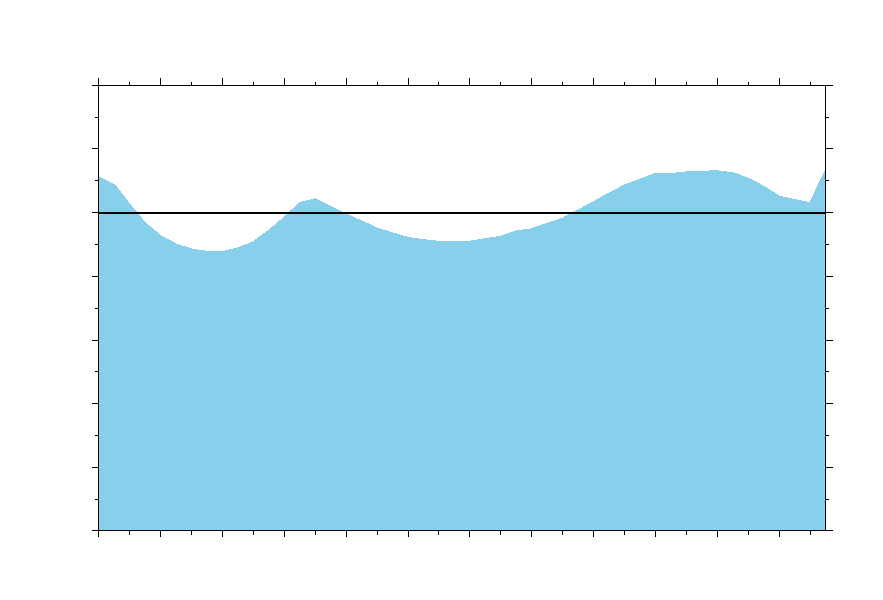
\includegraphics{plot_load_prof_summer_norm}}%
    \gplfronttext
  \end{picture}%
\endgroup
	& % GNUPLOT: LaTeX picture with Postscript
\begingroup
  \makeatletter
  \providecommand\color[2][]{%
    \GenericError{(gnuplot) \space\space\space\@spaces}{%
      Package color not loaded in conjunction with
      terminal option `colourtext'%
    }{See the gnuplot documentation for explanation.%
    }{Either use 'blacktext' in gnuplot or load the package
      color.sty in LaTeX.}%
    \renewcommand\color[2][]{}%
  }%
  \providecommand\includegraphics[2][]{%
    \GenericError{(gnuplot) \space\space\space\@spaces}{%
      Package graphicx or graphics not loaded%
    }{See the gnuplot documentation for explanation.%
    }{The gnuplot epslatex terminal needs graphicx.sty or graphics.sty.}%
    \renewcommand\includegraphics[2][]{}%
  }%
  \providecommand\rotatebox[2]{#2}%
  \@ifundefined{ifGPcolor}{%
    \newif\ifGPcolor
    \GPcolorfalse
  }{}%
  \@ifundefined{ifGPblacktext}{%
    \newif\ifGPblacktext
    \GPblacktexttrue
  }{}%
  % define a \g@addto@macro without @ in the name:
  \let\gplgaddtomacro\g@addto@macro
  % define empty templates for all commands taking text:
  \gdef\gplbacktext{}%
  \gdef\gplfronttext{}%
  \makeatother
  \ifGPblacktext
    % no textcolor at all
    \def\colorrgb#1{}%
    \def\colorgray#1{}%
  \else
    % gray or color?
    \ifGPcolor
      \def\colorrgb#1{\color[rgb]{#1}}%
      \def\colorgray#1{\color[gray]{#1}}%
      \expandafter\def\csname LTw\endcsname{\color{white}}%
      \expandafter\def\csname LTb\endcsname{\color{black}}%
      \expandafter\def\csname LTa\endcsname{\color{black}}%
      \expandafter\def\csname LT0\endcsname{\color[rgb]{1,0,0}}%
      \expandafter\def\csname LT1\endcsname{\color[rgb]{0,1,0}}%
      \expandafter\def\csname LT2\endcsname{\color[rgb]{0,0,1}}%
      \expandafter\def\csname LT3\endcsname{\color[rgb]{1,0,1}}%
      \expandafter\def\csname LT4\endcsname{\color[rgb]{0,1,1}}%
      \expandafter\def\csname LT5\endcsname{\color[rgb]{1,1,0}}%
      \expandafter\def\csname LT6\endcsname{\color[rgb]{0,0,0}}%
      \expandafter\def\csname LT7\endcsname{\color[rgb]{1,0.3,0}}%
      \expandafter\def\csname LT8\endcsname{\color[rgb]{0.5,0.5,0.5}}%
    \else
      % gray
      \def\colorrgb#1{\color{black}}%
      \def\colorgray#1{\color[gray]{#1}}%
      \expandafter\def\csname LTw\endcsname{\color{white}}%
      \expandafter\def\csname LTb\endcsname{\color{black}}%
      \expandafter\def\csname LTa\endcsname{\color{black}}%
      \expandafter\def\csname LT0\endcsname{\color{black}}%
      \expandafter\def\csname LT1\endcsname{\color{black}}%
      \expandafter\def\csname LT2\endcsname{\color{black}}%
      \expandafter\def\csname LT3\endcsname{\color{black}}%
      \expandafter\def\csname LT4\endcsname{\color{black}}%
      \expandafter\def\csname LT5\endcsname{\color{black}}%
      \expandafter\def\csname LT6\endcsname{\color{black}}%
      \expandafter\def\csname LT7\endcsname{\color{black}}%
      \expandafter\def\csname LT8\endcsname{\color{black}}%
    \fi
  \fi
    \setlength{\unitlength}{0.0500bp}%
    \ifx\gptboxheight\undefined%
      \newlength{\gptboxheight}%
      \newlength{\gptboxwidth}%
      \newsavebox{\gptboxtext}%
    \fi%
    \setlength{\fboxrule}{0.5pt}%
    \setlength{\fboxsep}{1pt}%
\begin{picture}(8162.00,5442.00)%
    \gplgaddtomacro\gplbacktext{%
      \csname LTb\endcsname%
      \put(594,503){\makebox(0,0)[r]{\strut{}0.0}}%
      \put(594,1114){\makebox(0,0)[r]{\strut{}0.2}}%
      \put(594,1725){\makebox(0,0)[r]{\strut{}0.4}}%
      \put(594,2336){\makebox(0,0)[r]{\strut{}0.6}}%
      \put(594,2948){\makebox(0,0)[r]{\strut{}0.8}}%
      \put(594,3559){\makebox(0,0)[r]{\strut{}1.0}}%
      \put(594,4170){\makebox(0,0)[r]{\strut{}1.2}}%
      \put(594,4781){\makebox(0,0)[r]{\strut{}1.4}}%
      \put(789,220){\makebox(0,0){\strut{}00:00}}%
      \put(1383,220){\makebox(0,0){\strut{}02:00}}%
      \put(1976,220){\makebox(0,0){\strut{}04:00}}%
      \put(2570,220){\makebox(0,0){\strut{}06:00}}%
      \put(3164,220){\makebox(0,0){\strut{}08:00}}%
      \put(3758,220){\makebox(0,0){\strut{}10:00}}%
      \put(4351,220){\makebox(0,0){\strut{}12:00}}%
      \put(4945,220){\makebox(0,0){\strut{}14:00}}%
      \put(5539,220){\makebox(0,0){\strut{}16:00}}%
      \put(6132,220){\makebox(0,0){\strut{}18:00}}%
      \put(6726,220){\makebox(0,0){\strut{}20:00}}%
      \put(7320,220){\makebox(0,0){\strut{}22:00}}%
    }%
    \gplgaddtomacro\gplfronttext{%
      \csname LTb\endcsname%
      \put(4277,5111){\makebox(0,0){\strut{}Normalised winter load profile}}%
    }%
    \gplbacktext
    \put(0,0){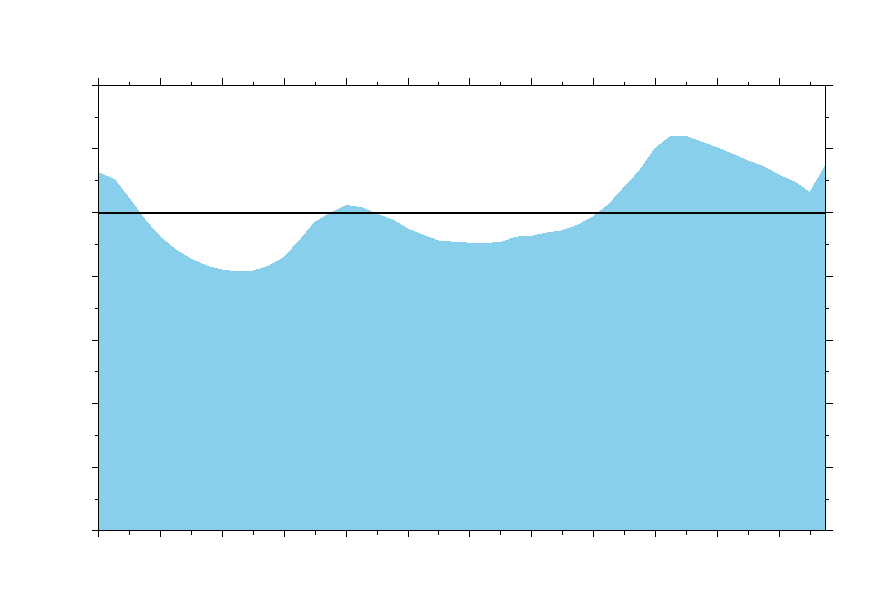
\includegraphics{plot_load_prof_winter_norm}}%
    \gplfronttext
  \end{picture}%
\endgroup

	\end{tabular}
	}
\end{figure}

Computer simulations generate control signals for $N$~=~105,408 5-minute dispatch intervals from 1 April 2015 to 31 March 2016.  It follows that the conversion factor from MW to MWh for a 5-minute dispatch interval, $\mwmwh = \tfrac{5}{60} = \tfrac{1}{12}$.  In the state-space model, process outputs $e(t\!+\!1)$ and $p_{d}(t\!+\!1)$ depend on control signals $p_{b+}(t)$, $p_{b-}(t)$ and $p_{w}(t)$.  Simulations of the na\"ive strategy minimise the tracking error of power dispatched to the grid, $p_{d}(t\!+\!1)$, relative to a couple of reference signals representing target baseload power:
\begin{itemize}
	\item  A constant set point in the range from 0.10~p.u.\ to 0.60~p.u.\ for each dispatch interval.\footnote{
The capacity factor for semi-scheduled wind farms in South Australia during fiscal year 2015 averaged 33.4\%, in the middle of the target baseload power range.  \textit{Capacity factor} is defined as the output of generating units, averaged over time,  expressed as a percentage of rated output or registered capacity.
}
	\item  A set point for each dispatch interval that follows the daily load profile of the season\footnote{
Load profiles, assuming 50\% probability of exceedance, for typical summer and winter days in fiscal year 2015 are generated using actual and forecast half-hourly demand data accessible through AEMO's web-based portal \citep{NEFR15b}.  For seasonal analyses, AEMO classifies the months from October to March as summer, and the months from April to September as winter.
} with its average in the range from 0.10~p.u.\ to 0.60~p.u.
\end{itemize}
Figure~\ref{fig:load_prof_norm} plots the normalised load profiles for typical summer and winter days in SA during fiscal year 2015 --- the average load during a typical summer or winter day is equal to 1.0.  In these simulations, performance index~\eqref{eqn:quad_cost_func} does not penalise the tracking error of SOC of the battery, $e(t\!+\!1)$, relative to its reference signal, nor does it penalise control effort, $\boldsymbol{\Delta{u}}(t)$.  That is, the odd diagonal elements of $\Omega$ are set to zero, and $\lambda = 0$.  With respect to the control signals, wind power generation command, $p_{w}(t)$, is set to the corresponding UIGF forecast, and optimisation of the process control law determines the battery charge command, $p_{b+}(t)$, and battery discharge command, $p_{b-}(t)$.\footnote{
Optimisation of the process control law employs mixed integer quadratic program \texttt{cplexmiqp()} from the CPLEX for MATLAB Toolbox.
}

\begin{figure}[!t]
	\centering
	\caption[Dispatchability of wind power with battery energy storage --- set point is fixed to a constant value]{Probability of (wind and battery) power dispatched to the grid equaling or exceeding the reference signal, or set point, representing target baseload power.  The reference signal is fixed to a constant value in the target baseload power range.  The MPC controller uses 5-minute dispatch data, published by AEMO, from 1 April 2015 to 31 March 2016.  Registered generation capacity of the wind farm is 1.0 p.u.  Specifications of utility-scale, lithium-ion batteries are reported in Table~\ref{tbl:bess_specs}.} 
	\label{fig:disp_wind_bess_flat}
	\scalebox{0.90}{
		% GNUPLOT: LaTeX picture with Postscript
\begingroup
  \makeatletter
  \providecommand\color[2][]{%
    \GenericError{(gnuplot) \space\space\space\@spaces}{%
      Package color not loaded in conjunction with
      terminal option `colourtext'%
    }{See the gnuplot documentation for explanation.%
    }{Either use 'blacktext' in gnuplot or load the package
      color.sty in LaTeX.}%
    \renewcommand\color[2][]{}%
  }%
  \providecommand\includegraphics[2][]{%
    \GenericError{(gnuplot) \space\space\space\@spaces}{%
      Package graphicx or graphics not loaded%
    }{See the gnuplot documentation for explanation.%
    }{The gnuplot epslatex terminal needs graphicx.sty or graphics.sty.}%
    \renewcommand\includegraphics[2][]{}%
  }%
  \providecommand\rotatebox[2]{#2}%
  \@ifundefined{ifGPcolor}{%
    \newif\ifGPcolor
    \GPcolorfalse
  }{}%
  \@ifundefined{ifGPblacktext}{%
    \newif\ifGPblacktext
    \GPblacktexttrue
  }{}%
  % define a \g@addto@macro without @ in the name:
  \let\gplgaddtomacro\g@addto@macro
  % define empty templates for all commands taking text:
  \gdef\gplbacktext{}%
  \gdef\gplfronttext{}%
  \makeatother
  \ifGPblacktext
    % no textcolor at all
    \def\colorrgb#1{}%
    \def\colorgray#1{}%
  \else
    % gray or color?
    \ifGPcolor
      \def\colorrgb#1{\color[rgb]{#1}}%
      \def\colorgray#1{\color[gray]{#1}}%
      \expandafter\def\csname LTw\endcsname{\color{white}}%
      \expandafter\def\csname LTb\endcsname{\color{black}}%
      \expandafter\def\csname LTa\endcsname{\color{black}}%
      \expandafter\def\csname LT0\endcsname{\color[rgb]{1,0,0}}%
      \expandafter\def\csname LT1\endcsname{\color[rgb]{0,1,0}}%
      \expandafter\def\csname LT2\endcsname{\color[rgb]{0,0,1}}%
      \expandafter\def\csname LT3\endcsname{\color[rgb]{1,0,1}}%
      \expandafter\def\csname LT4\endcsname{\color[rgb]{0,1,1}}%
      \expandafter\def\csname LT5\endcsname{\color[rgb]{1,1,0}}%
      \expandafter\def\csname LT6\endcsname{\color[rgb]{0,0,0}}%
      \expandafter\def\csname LT7\endcsname{\color[rgb]{1,0.3,0}}%
      \expandafter\def\csname LT8\endcsname{\color[rgb]{0.5,0.5,0.5}}%
    \else
      % gray
      \def\colorrgb#1{\color{black}}%
      \def\colorgray#1{\color[gray]{#1}}%
      \expandafter\def\csname LTw\endcsname{\color{white}}%
      \expandafter\def\csname LTb\endcsname{\color{black}}%
      \expandafter\def\csname LTa\endcsname{\color{black}}%
      \expandafter\def\csname LT0\endcsname{\color{black}}%
      \expandafter\def\csname LT1\endcsname{\color{black}}%
      \expandafter\def\csname LT2\endcsname{\color{black}}%
      \expandafter\def\csname LT3\endcsname{\color{black}}%
      \expandafter\def\csname LT4\endcsname{\color{black}}%
      \expandafter\def\csname LT5\endcsname{\color{black}}%
      \expandafter\def\csname LT6\endcsname{\color{black}}%
      \expandafter\def\csname LT7\endcsname{\color{black}}%
      \expandafter\def\csname LT8\endcsname{\color{black}}%
    \fi
  \fi
    \setlength{\unitlength}{0.0500bp}%
    \ifx\gptboxheight\undefined%
      \newlength{\gptboxheight}%
      \newlength{\gptboxwidth}%
      \newsavebox{\gptboxtext}%
    \fi%
    \setlength{\fboxrule}{0.5pt}%
    \setlength{\fboxsep}{1pt}%
\begin{picture}(8162.00,5442.00)%
    \gplgaddtomacro\gplbacktext{%
      \csname LTb\endcsname%
      \put(814,704){\makebox(0,0)[r]{\strut{}0}}%
      \put(814,1151){\makebox(0,0)[r]{\strut{}10}}%
      \put(814,1599){\makebox(0,0)[r]{\strut{}20}}%
      \put(814,2046){\makebox(0,0)[r]{\strut{}30}}%
      \put(814,2493){\makebox(0,0)[r]{\strut{}40}}%
      \put(814,2941){\makebox(0,0)[r]{\strut{}50}}%
      \put(814,3388){\makebox(0,0)[r]{\strut{}60}}%
      \put(814,3835){\makebox(0,0)[r]{\strut{}70}}%
      \put(814,4282){\makebox(0,0)[r]{\strut{}80}}%
      \put(814,4730){\makebox(0,0)[r]{\strut{}90}}%
      \put(814,5177){\makebox(0,0)[r]{\strut{}100}}%
      \put(946,484){\makebox(0,0){\strut{}0.00}}%
      \put(1920,484){\makebox(0,0){\strut{}0.10}}%
      \put(2894,484){\makebox(0,0){\strut{}0.20}}%
      \put(3868,484){\makebox(0,0){\strut{}0.30}}%
      \put(4843,484){\makebox(0,0){\strut{}0.40}}%
      \put(5817,484){\makebox(0,0){\strut{}0.50}}%
      \put(6791,484){\makebox(0,0){\strut{}0.60}}%
      \put(7765,484){\makebox(0,0){\strut{}0.70}}%
    }%
    \gplgaddtomacro\gplfronttext{%
      \csname LTb\endcsname%
      \put(176,2940){\rotatebox{-270}{\makebox(0,0){\strut{}$\P\left(\text{power dispatched} \geq \text{reference signal}\right)$, \%}}}%
      \put(4355,154){\makebox(0,0){\strut{}Reference signal for power dispatched to the grid, p.u.}}%
      \csname LTb\endcsname%
      \put(1948,1712){\makebox(0,0)[l]{\strut{}No energy storage}}%
      \csname LTb\endcsname%
      \put(1948,1492){\makebox(0,0)[l]{\strut{}Battery (1), capacity = 0.50 p.u.}}%
      \csname LTb\endcsname%
      \put(1948,1272){\makebox(0,0)[l]{\strut{}Battery (2), capacity = 0.75 p.u.}}%
      \csname LTb\endcsname%
      \put(1948,1052){\makebox(0,0)[l]{\strut{}Battery (3), capacity = 1.00 p.u.}}%
    }%
    \gplbacktext
    \put(0,0){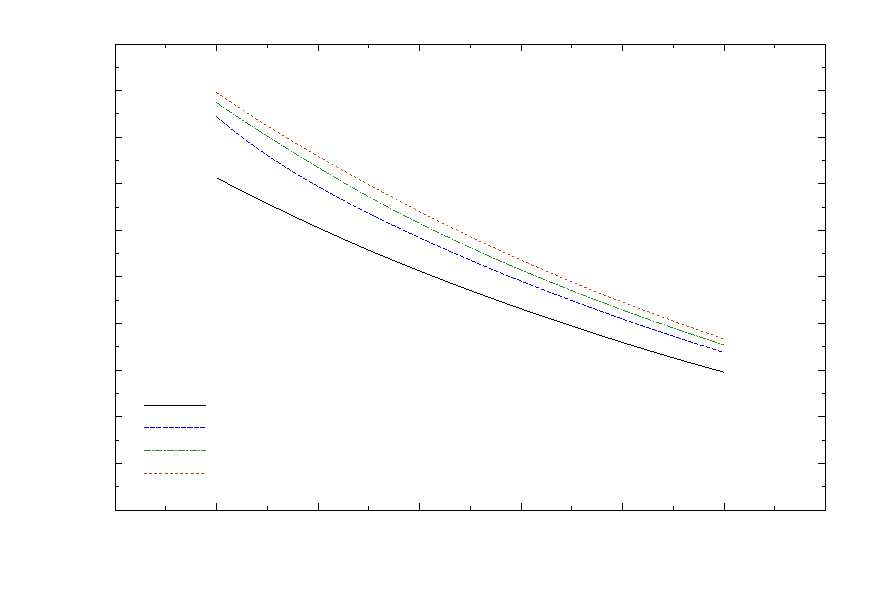
\includegraphics{plot_disp_wind_bess_flat}}%
    \gplfronttext
  \end{picture}%
\endgroup

	}
\end{figure}

Figures~\ref{fig:disp_wind_bess_flat} and \ref{fig:disp_wind_bess_load_prof} illustrate the improvement in wind power dispatch with battery energy storage relative to no energy storage by plotting the probability of power dispatched to the grid equaling or exceeding the reference signal representing target baseload power.  In the former the reference signal is fixed to a constant value, while in the latter it follows the daily load profile of the season.  The results, plotted in Figures~\ref{fig:disp_wind_bess_flat} and \ref{fig:disp_wind_bess_load_prof}, are not significantly different.  Over the target baseload power range from 0.10~p.u.\ to 0.60~p.u., the probability of power dispatched to the grid equaling or exceeding the reference signal is between 15\% and 25\% higher with a utility-scale battery than with no energy storage.  Clearly, the magnitude of the improvement in the dispatchability of wind power with battery energy storage depends on the specifications of the battery.  But, even on today's utility scale, battery power can only substitute for a fraction of the power generated by a commercial wind farm for a limited time.  For example, a utility-scale battery with energy capacity of 0.50 p.u.\ and power rating of 0.175 p.u.\ subjected to a 70\% discharge cycle can only supply electricity at its rated power for two hours.

\begin{figure}[!t]
	\centering
	\caption[Dispatchability of wind power with battery energy storage --- set point follows the daily load profile of the season]{Probability of (wind and battery) power dispatched to the grid equaling or exceeding the reference signal, or set point, representing target baseload power.  The reference signal follows the daily load profile of the season with its average in the target baseload power range. The MPC controller uses 5-minute dispatch data, published by AEMO, from 1 April 2015 to 31 March 2016.  Registered generation capacity of the wind farm is 1.0 p.u.  Specifications of utility-scale, lithium-ion batteries are reported in Table~\ref{tbl:bess_specs}.} 
	\label{fig:disp_wind_bess_load_prof}
	\scalebox{0.90}{
		% GNUPLOT: LaTeX picture with Postscript
\begingroup
  \makeatletter
  \providecommand\color[2][]{%
    \GenericError{(gnuplot) \space\space\space\@spaces}{%
      Package color not loaded in conjunction with
      terminal option `colourtext'%
    }{See the gnuplot documentation for explanation.%
    }{Either use 'blacktext' in gnuplot or load the package
      color.sty in LaTeX.}%
    \renewcommand\color[2][]{}%
  }%
  \providecommand\includegraphics[2][]{%
    \GenericError{(gnuplot) \space\space\space\@spaces}{%
      Package graphicx or graphics not loaded%
    }{See the gnuplot documentation for explanation.%
    }{The gnuplot epslatex terminal needs graphicx.sty or graphics.sty.}%
    \renewcommand\includegraphics[2][]{}%
  }%
  \providecommand\rotatebox[2]{#2}%
  \@ifundefined{ifGPcolor}{%
    \newif\ifGPcolor
    \GPcolorfalse
  }{}%
  \@ifundefined{ifGPblacktext}{%
    \newif\ifGPblacktext
    \GPblacktexttrue
  }{}%
  % define a \g@addto@macro without @ in the name:
  \let\gplgaddtomacro\g@addto@macro
  % define empty templates for all commands taking text:
  \gdef\gplbacktext{}%
  \gdef\gplfronttext{}%
  \makeatother
  \ifGPblacktext
    % no textcolor at all
    \def\colorrgb#1{}%
    \def\colorgray#1{}%
  \else
    % gray or color?
    \ifGPcolor
      \def\colorrgb#1{\color[rgb]{#1}}%
      \def\colorgray#1{\color[gray]{#1}}%
      \expandafter\def\csname LTw\endcsname{\color{white}}%
      \expandafter\def\csname LTb\endcsname{\color{black}}%
      \expandafter\def\csname LTa\endcsname{\color{black}}%
      \expandafter\def\csname LT0\endcsname{\color[rgb]{1,0,0}}%
      \expandafter\def\csname LT1\endcsname{\color[rgb]{0,1,0}}%
      \expandafter\def\csname LT2\endcsname{\color[rgb]{0,0,1}}%
      \expandafter\def\csname LT3\endcsname{\color[rgb]{1,0,1}}%
      \expandafter\def\csname LT4\endcsname{\color[rgb]{0,1,1}}%
      \expandafter\def\csname LT5\endcsname{\color[rgb]{1,1,0}}%
      \expandafter\def\csname LT6\endcsname{\color[rgb]{0,0,0}}%
      \expandafter\def\csname LT7\endcsname{\color[rgb]{1,0.3,0}}%
      \expandafter\def\csname LT8\endcsname{\color[rgb]{0.5,0.5,0.5}}%
    \else
      % gray
      \def\colorrgb#1{\color{black}}%
      \def\colorgray#1{\color[gray]{#1}}%
      \expandafter\def\csname LTw\endcsname{\color{white}}%
      \expandafter\def\csname LTb\endcsname{\color{black}}%
      \expandafter\def\csname LTa\endcsname{\color{black}}%
      \expandafter\def\csname LT0\endcsname{\color{black}}%
      \expandafter\def\csname LT1\endcsname{\color{black}}%
      \expandafter\def\csname LT2\endcsname{\color{black}}%
      \expandafter\def\csname LT3\endcsname{\color{black}}%
      \expandafter\def\csname LT4\endcsname{\color{black}}%
      \expandafter\def\csname LT5\endcsname{\color{black}}%
      \expandafter\def\csname LT6\endcsname{\color{black}}%
      \expandafter\def\csname LT7\endcsname{\color{black}}%
      \expandafter\def\csname LT8\endcsname{\color{black}}%
    \fi
  \fi
    \setlength{\unitlength}{0.0500bp}%
    \ifx\gptboxheight\undefined%
      \newlength{\gptboxheight}%
      \newlength{\gptboxwidth}%
      \newsavebox{\gptboxtext}%
    \fi%
    \setlength{\fboxrule}{0.5pt}%
    \setlength{\fboxsep}{1pt}%
\begin{picture}(8162.00,5442.00)%
    \gplgaddtomacro\gplbacktext{%
      \csname LTb\endcsname%
      \put(814,704){\makebox(0,0)[r]{\strut{}0}}%
      \put(814,1151){\makebox(0,0)[r]{\strut{}10}}%
      \put(814,1599){\makebox(0,0)[r]{\strut{}20}}%
      \put(814,2046){\makebox(0,0)[r]{\strut{}30}}%
      \put(814,2493){\makebox(0,0)[r]{\strut{}40}}%
      \put(814,2941){\makebox(0,0)[r]{\strut{}50}}%
      \put(814,3388){\makebox(0,0)[r]{\strut{}60}}%
      \put(814,3835){\makebox(0,0)[r]{\strut{}70}}%
      \put(814,4282){\makebox(0,0)[r]{\strut{}80}}%
      \put(814,4730){\makebox(0,0)[r]{\strut{}90}}%
      \put(814,5177){\makebox(0,0)[r]{\strut{}100}}%
      \put(946,484){\makebox(0,0){\strut{}0.00}}%
      \put(1920,484){\makebox(0,0){\strut{}0.10}}%
      \put(2894,484){\makebox(0,0){\strut{}0.20}}%
      \put(3868,484){\makebox(0,0){\strut{}0.30}}%
      \put(4843,484){\makebox(0,0){\strut{}0.40}}%
      \put(5817,484){\makebox(0,0){\strut{}0.50}}%
      \put(6791,484){\makebox(0,0){\strut{}0.60}}%
      \put(7765,484){\makebox(0,0){\strut{}0.70}}%
    }%
    \gplgaddtomacro\gplfronttext{%
      \csname LTb\endcsname%
      \put(176,2940){\rotatebox{-270}{\makebox(0,0){\strut{}$\P\left(\text{power dispatched} \geq \text{reference signal}\right)$, \%}}}%
      \put(4355,154){\makebox(0,0){\strut{}Average of reference signal for power dispatched to the grid, p.u.}}%
      \csname LTb\endcsname%
      \put(1948,1712){\makebox(0,0)[l]{\strut{}No energy storage}}%
      \csname LTb\endcsname%
      \put(1948,1492){\makebox(0,0)[l]{\strut{}Battery (1), capacity = 0.50 p.u.}}%
      \csname LTb\endcsname%
      \put(1948,1272){\makebox(0,0)[l]{\strut{}Battery (2), capacity = 0.75 p.u.}}%
      \csname LTb\endcsname%
      \put(1948,1052){\makebox(0,0)[l]{\strut{}Battery (3), capacity = 1.00 p.u.}}%
    }%
    \gplbacktext
    \put(0,0){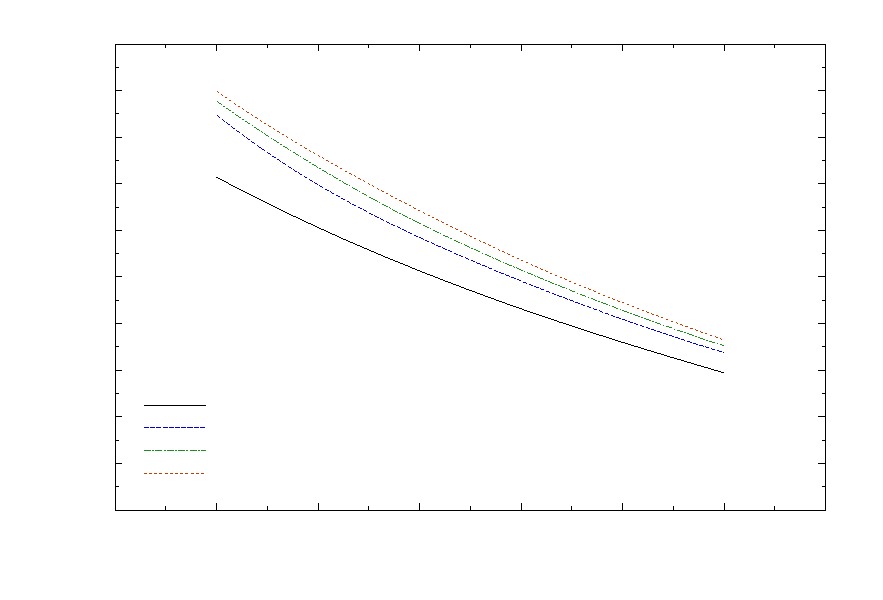
\includegraphics{plot_disp_wind_bess_load_prof}}%
    \gplfronttext
  \end{picture}%
\endgroup

	}
\end{figure}

We remark that this paper does not attempt to make the economic case for installing utility-scale batteries to facilitate time shifting of wind power dispatched to the grid.  But, as the cost of battery energy storage continues to tumble, utility-scale batteries may become commercially viable in the near- to medium-term.

\begin{figure}[!t]
	\centering
	\caption[Wind power generated in SA during December 2015]{Wind power generated in South Australia at 5-minute intervals during December 2015.  Each day of the month is plotted in a different colour.	\protect\\
		{\footnotesize Source: Australian Energy Market Operator.}} 
	\label{fig:wind_gen_1512}
	\scalebox{0.90}{
		% GNUPLOT: LaTeX picture with Postscript
\begingroup
  \makeatletter
  \providecommand\color[2][]{%
    \GenericError{(gnuplot) \space\space\space\@spaces}{%
      Package color not loaded in conjunction with
      terminal option `colourtext'%
    }{See the gnuplot documentation for explanation.%
    }{Either use 'blacktext' in gnuplot or load the package
      color.sty in LaTeX.}%
    \renewcommand\color[2][]{}%
  }%
  \providecommand\includegraphics[2][]{%
    \GenericError{(gnuplot) \space\space\space\@spaces}{%
      Package graphicx or graphics not loaded%
    }{See the gnuplot documentation for explanation.%
    }{The gnuplot epslatex terminal needs graphicx.sty or graphics.sty.}%
    \renewcommand\includegraphics[2][]{}%
  }%
  \providecommand\rotatebox[2]{#2}%
  \@ifundefined{ifGPcolor}{%
    \newif\ifGPcolor
    \GPcolorfalse
  }{}%
  \@ifundefined{ifGPblacktext}{%
    \newif\ifGPblacktext
    \GPblacktexttrue
  }{}%
  % define a \g@addto@macro without @ in the name:
  \let\gplgaddtomacro\g@addto@macro
  % define empty templates for all commands taking text:
  \gdef\gplbacktext{}%
  \gdef\gplfronttext{}%
  \makeatother
  \ifGPblacktext
    % no textcolor at all
    \def\colorrgb#1{}%
    \def\colorgray#1{}%
  \else
    % gray or color?
    \ifGPcolor
      \def\colorrgb#1{\color[rgb]{#1}}%
      \def\colorgray#1{\color[gray]{#1}}%
      \expandafter\def\csname LTw\endcsname{\color{white}}%
      \expandafter\def\csname LTb\endcsname{\color{black}}%
      \expandafter\def\csname LTa\endcsname{\color{black}}%
      \expandafter\def\csname LT0\endcsname{\color[rgb]{1,0,0}}%
      \expandafter\def\csname LT1\endcsname{\color[rgb]{0,1,0}}%
      \expandafter\def\csname LT2\endcsname{\color[rgb]{0,0,1}}%
      \expandafter\def\csname LT3\endcsname{\color[rgb]{1,0,1}}%
      \expandafter\def\csname LT4\endcsname{\color[rgb]{0,1,1}}%
      \expandafter\def\csname LT5\endcsname{\color[rgb]{1,1,0}}%
      \expandafter\def\csname LT6\endcsname{\color[rgb]{0,0,0}}%
      \expandafter\def\csname LT7\endcsname{\color[rgb]{1,0.3,0}}%
      \expandafter\def\csname LT8\endcsname{\color[rgb]{0.5,0.5,0.5}}%
    \else
      % gray
      \def\colorrgb#1{\color{black}}%
      \def\colorgray#1{\color[gray]{#1}}%
      \expandafter\def\csname LTw\endcsname{\color{white}}%
      \expandafter\def\csname LTb\endcsname{\color{black}}%
      \expandafter\def\csname LTa\endcsname{\color{black}}%
      \expandafter\def\csname LT0\endcsname{\color{black}}%
      \expandafter\def\csname LT1\endcsname{\color{black}}%
      \expandafter\def\csname LT2\endcsname{\color{black}}%
      \expandafter\def\csname LT3\endcsname{\color{black}}%
      \expandafter\def\csname LT4\endcsname{\color{black}}%
      \expandafter\def\csname LT5\endcsname{\color{black}}%
      \expandafter\def\csname LT6\endcsname{\color{black}}%
      \expandafter\def\csname LT7\endcsname{\color{black}}%
      \expandafter\def\csname LT8\endcsname{\color{black}}%
    \fi
  \fi
    \setlength{\unitlength}{0.0500bp}%
    \ifx\gptboxheight\undefined%
      \newlength{\gptboxheight}%
      \newlength{\gptboxwidth}%
      \newsavebox{\gptboxtext}%
    \fi%
    \setlength{\fboxrule}{0.5pt}%
    \setlength{\fboxsep}{1pt}%
\begin{picture}(8162.00,5442.00)%
    \gplgaddtomacro\gplbacktext{%
      \csname LTb\endcsname%
      \put(740,400){\makebox(0,0)[r]{\strut{}0}}%
      \put(740,1200){\makebox(0,0)[r]{\strut{}20}}%
      \put(740,2000){\makebox(0,0)[r]{\strut{}40}}%
      \put(740,2801){\makebox(0,0)[r]{\strut{}60}}%
      \put(740,3601){\makebox(0,0)[r]{\strut{}80}}%
      \put(740,4401){\makebox(0,0)[r]{\strut{}100}}%
      \put(740,5201){\makebox(0,0)[r]{\strut{}120}}%
      \put(860,200){\makebox(0,0){\strut{}00:00}}%
      \put(1438,200){\makebox(0,0){\strut{}02:00}}%
      \put(2017,200){\makebox(0,0){\strut{}04:00}}%
      \put(2595,200){\makebox(0,0){\strut{}06:00}}%
      \put(3174,200){\makebox(0,0){\strut{}08:00}}%
      \put(3752,200){\makebox(0,0){\strut{}10:00}}%
      \put(4331,200){\makebox(0,0){\strut{}12:00}}%
      \put(4909,200){\makebox(0,0){\strut{}14:00}}%
      \put(5487,200){\makebox(0,0){\strut{}16:00}}%
      \put(6066,200){\makebox(0,0){\strut{}18:00}}%
      \put(6644,200){\makebox(0,0){\strut{}20:00}}%
      \put(7223,200){\makebox(0,0){\strut{}22:00}}%
      \put(7801,200){\makebox(0,0){\strut{}00:00}}%
    }%
    \gplgaddtomacro\gplfronttext{%
      \csname LTb\endcsname%
      \put(160,2800){\rotatebox{-270}{\makebox(0,0){\strut{}MWh}}}%
      \csname LTb\endcsname%
      \put(1763,5038){\makebox(0,0)[l]{\strut{}Average}}%
    }%
    \gplbacktext
    \put(0,0){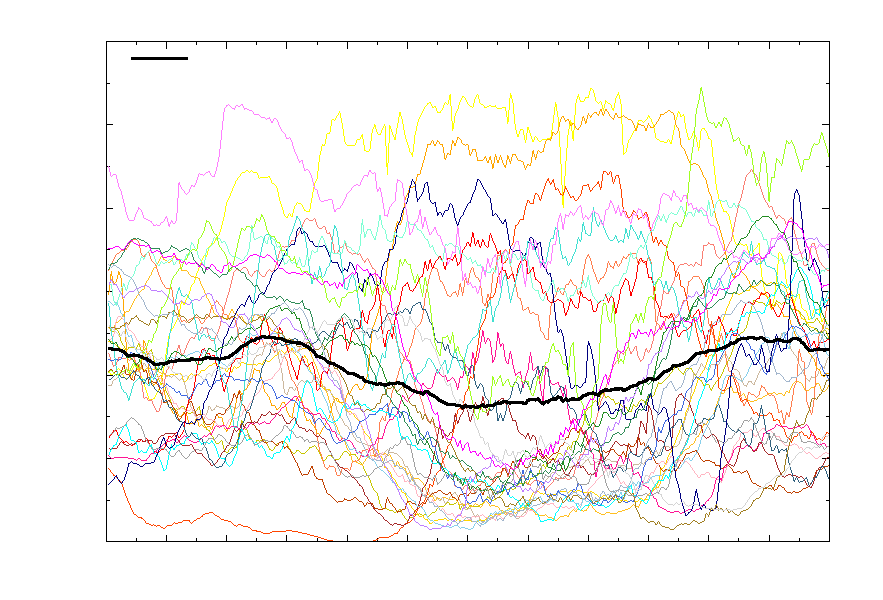
\includegraphics{plot_wind_gen_1512}}%
    \gplfronttext
  \end{picture}%
\endgroup

	}
\end{figure}

As noted previously, the simulations reported in this paper implement a na\"ive strategy with single-period prediction and control horizons.  A more sophisticated strategy would store excess renewable energy during periods of low demand, and discharge the stored energy for dispatch to the grid during periods of high demand, say, between 4:00~pm and 9:00~pm.  This latter strategy requires UIGF forecasts determined by AWEFS over a prediction horizon covering the pre-dispatch period\footnote{
The trading day comprises 48 half-hourly periods commencing from the 04:00:01--04:30:00 trading interval, designated by the end time of the period, that is, the 4:30 am trading interval.  The 40-hour pre-dispatch period commences with the 12:30 pm trading interval on the day before the actual trading day to which the dispatch offers apply \citeyearpar[AEMO,][]{AEMO10}.
} to generate a sequence of $n_{y}$ reference signals for power dispatched to the grid that applies over an $n_{u}$-period (i.e., multi-period) control horizon.  Presumably prices would be higher during peak demand periods, so time shifting of wind power dispatched to the grid would fetch higher revenue for the wind generator owner/operator.  Moveover, if AEMO's pre-dispatch and dispatch process \citeyearpar[AEMO,][]{AEMO10} permitted wind generators to submit their dispatch offers with the quantity of electrical power for sale by price band, as conventional generators do, then wind generators could schedule power dispatched to the grid taking into account UIGF forecasts and SOC of the battery coupled to the wind farm.  The time series of power scheduled for dispatch would then become the reference signal of the MPC controller.

AWEFS produces UIGF forecasts over a range of horizons with varying resolutions at different frequencies \citeyearpar[AEMO,][]{AEMO14b}: dispatch (5-minute horizon, 5-minute resolution, and 5-minute frequency); 5-minute pre-dispatch (2-hour horizon, 5-minute resolution, and 5-minute frequency); and pre-dispatch (up to 40-hour horizon, 30-minute resolution, and 30-minute frequency).  While charts such as Figure~\ref{fig:wind_gen_1512} are often used to demonstrate the difficulty in forecasting wind power generation, the monthly average of the normalised mean absolute error of forecasts\footnote{
The normalised mean absolute error is calculated as the absolute difference between forecast and actual generation, divided by the registered generation capacity.
} was less than 8.2\% for forecast horizons up to 40 hours, and less than 1.5\% for the 5-minute forecast horizon during fiscal year 2015 \citeyearpar[AEMO,][]{SAWSR15}.  

%The incremental state-space MPC controller for wind power dispatch with battery energy storage described in Section~\ref{sect:ssmpc_dispatch} is an implementation of the classical approach.  However, stochastic MPC may be a more appropriate technique for modelling probabilistic constraints, such as dispatching a designated level of baseload power to the grid with a given level of confidence.

%===========================================================================================%
% CONCLUSION																				 %
%===========================================================================================%
\section{Conclusion}\label{sect:conclusion}
In this paper we formulate the process of wind power dispatch with battery energy storage as an incremental state-space model that properly accounts for the charge/discharge efficiency of the battery.  Furthermore, MPC based on an incremental state-space model allows the controller to penalise control effort, as well as the tracking error of process outputs relative to their reference signals.  Our empirical analysis implements this state-space MPC controller.  It simulates a na\"ive strategy for improving wind power dispatch with battery energy storage over one full year using 5-minute dispatch forecasts produced by AWEFS and published by AEMO.  We suppose that, subject to constraints on SOC, utility-scale batteries coupled to an SA wind farm can supply electricity at their rated power for two hours.  Repeating the computer simulations for these utility-scale batteries with varying power rating and energy capacity, we find that the probability of equaling or exceeding a target baseload power is between 15\% and 25\%.  

A more sophisticated strategy, which we leave for future research, would store excess renewable energy during periods of low demand, and discharge the stored energy for dispatch to the electricity grid during periods of high demand when, presumably, prices would be higher.  Wind generators could schedule power dispatched to the grid by taking into account UIGF forecasts and SOC of the battery, and accordingly submit their dispatch offers with the quantity of electrical power for sale by price band during pre-dispatch and dispatch.

Computer simulations of wind power dispatch with battery energy storage presented in this paper use classical MPC, which binds the process with hard constraints.  However, it may be more appropriate to model the process with probabilistic constraints, such as dispatching a designated level of baseload power to the grid with a given level of confidence.  If the uncertainty can be modelled as random with a known probability distribution, then stochastic MPC drives the process while satisfying such probabilistic constraints.  Future research could examine improvements in the dispatchability of intermittent renewable energy using stochastic MPC, a relatively undeveloped research area \citep[chap.~1]{KC16}.

The commercial viability of installing utility-scale batteries on wind farms may be achieved by targeting profits of energy arbitrage and payments for the provision of ancillary services.  While the former is evidently a financial transaction, the latter is crucial for ensuring power system reliability, that is, supplying quality power.\footnote{
The \citet[IEC 60050--617,][]{IEC617} defines \textit{quality power} as ``characteristics of the electric current, voltage and frequencies at a given point in an electric power system, evaluated against a set of reference technical parameters.''  Ancillary services assure the reliable transmission of quality power.	
}  As intermittent renewable energy generation displaces conventional generation and its penetration reaches the levels in SA, independent system operators are imposing requirements on wind power generators, in particular, to provide frequency (active power) and voltage (reactive power) control --- ancillary services historically supplied by conventional generators \citep{ABLFJD12}.  For example, grid codes in Denmark, Ireland and Spain require wind farms to accept ``delta control''  commands from the ISO to limit wind power generation below available capacity for dispatch by a fixed amount, in effect maintaining a spinning reserve available for frequency regulation \citep{ECAR11}.\footnote{
Power output of a wind turbine may be controlled by varying the generator load torque, blade pitch angle and rotor yaw angle \citep{ABLFJD12}.
}  But, maintaining a spinning reserve needlessly wastes wind energy and foregoes revenue from wind power generation.  Here, the time shifting capability enabled by battery energy storage would allow more efficient transformation of wind energy and higher revenue from wind power generation, while complying with grid code (i.e., ancillary services) requirements.
	
Microgrids offer the possibility of experimenting with satisfying the multiple objectives of supplying baseload power, ensuring power system reliability and profiting from energy arbitrage.  Note that the variability of intermittent renewable energy generation would be dampened in microgrids with wind turbines and solar PV panels.  MPC can be applied to balance the multiple objectives of a MIMO system by tuning the weighting coefficients assigned to tracking errors captured in the performance index.  Microgrids, with their distributed energy generation and storage, promise the additional economic benefit of deferring upgrades to transmission and distribution grids.  Therefore, the economic case for microgrids should consider savings from the deferment of network upgrades, which accrue initially to transmission and distribution network service providers, and ultimately to electricity consumers.

%===========================================================================================%
% REFERENCES																				 %
%===========================================================================================%
\bibliographystyle{chicago}
\bibliography{sagridnat}

\end{document}
